% \documentclass[runningheads]{llncs}
\documentclass[conference,a4paper]{IEEEtran}
\IEEEoverridecommandlockouts
\usepackage{luatextra}
\usepackage{currvita}
%
\usepackage{makeidx}  % allows for indexgeneration
\usepackage{url}
\usepackage[biblabel]{cite}
\usepackage{amsmath,amssymb,amsfonts}
\usepackage{algorithmic}
\usepackage{graphicx}
%\usepackage[pdftex]{graphicx}
%\usepackage[dvips]{graphicx}
\usepackage{alltt}
\usepackage{textcomp}
\usepackage{enumitem}
\usepackage{indentfirst}
\usepackage{doi}
\renewcommand{\doitext}{DOI:}

%
% Used for displaying a sample figure. If possible, figure files should
% be included in EPS format.
%
% If you use the hyperref package, please uncomment the following line
% to display URLs in blue roman font according to Springer's eBook style:
% \renewcommand\UrlFont{\color{blue}\rmfamily}


\usepackage{hyperref}
\hypersetup{
    % bookmarks=true,         % show bookmarks bar?
    unicode=true,          % non-Latin characters in Acrobat’s bookmarks
    pdftoolbar=true,        % show Acrobat’s toolbar?
    pdfmenubar=true,        % show Acrobat’s menu?
    pdffitwindow=false,     % window fit to page when opened
    pdfstartview={FitH},    % fits the width of the page to the window
    %pdftitle={},    % title
    %pdfauthor={Author},     % author
    %pdfsubject={Subject},   % subject of the document
    %pdfcreator={Creator},   % creator of the document
    %pdfproducer={Producer}, % producer of the document
    %pdfkeywords={keyword1, key2, key3}, % list of keywords
    %pdfnewwindow=true,      % links in new PDF window
    colorlinks=true,       % false: boxed links; true: colored links
    linkcolor=black,          % color of internal links (change box color with linkbordercolor)
    citecolor=black,        % color of links to bibliography
    filecolor=black,      % color of file links
    urlcolor=black,           % color of external links
    final=true
  }

\setmainfont{Times New Roman}

\begin{document}
%
\title{Information Technologies for Supporting Research of Complex Large-Scale Resource-Driven Discrete-Event Systems Under Uncertainty}
%
%\titlerunning{IT for complex large-scale DES under uncertainties}
% If the paper title is too long for the running head, you can set
% an abbreviated paper title here
%
\def\inst#1{${}^#1$}
\author{
% %\def\and{, }
\def\and{\unskip, }
\IEEEauthorblockN{Evgeny~Cherkashin\inst{1} \and
Qiumei~Cong\inst{2} \and
Igor~Bychkov\inst{1} \and
Nadezhda~Nagul\inst{1} \and
Artem~Davydov\inst{1} \and
Yue~Wang\inst{2} \and
Shi~Huiyuan\inst{2}}
%
%\authorrunning{E. Cherkashin, Q. Cong, I. Bychkov, N. Nagul, A. Davydov, Y. Wang, Sh. Huiyuan} % abbreviated author list (for running head)
%
%%%% list of authors for the TOC (use if author list has to be modified)
%\tocauthor{Alexey Shigarov, Vasiliy Khristyuk, and Evgeniy Cherkashin}

%\tocauthor{Evgeny Cherkashin, Quimey Cong, Igor Bychkov \emph{et al.}}

\IEEEauthorblockA{\inst{1}~\textit{Matrosov Institute for System Dynamics and Control Theory of SB RAS}, Irkutsk, Russia\\
eugeneai@icc.ru}
\IEEEauthorblockA{\inst{2}~\textit{Liaoning Shihua University, School of Information and Control Engineering,} Fushun, China\\
cong\_0828@163.com}%,\\ WWW home page: \texttt{http://td.icc.ru}
}
%


\maketitle              % typeset the header of the contribution
%
\begin{abstract}
  The paper states basic ideas of an approach dealing with uncertainties in models of manufacturing process of an industrial scale. The models are complexes including discrete-event systems representing the manufacturing schedule and resource-driven game description of its behavior in a competitive multi-agent environment. The model object is a subject of control on various levels. Due to the large scale of the object, the control is synthesized as a result of a logical inference, either a theorem proving or forward-chaining modeling a computer simulation scenarios analysis. The uncertainties appear in the model due to activities of competitors or internal factors having probabilistic nature and represented as internal events or shortage of resources. The synthesized control should ensure that the system corresponds to a set of predefined constraints and/or maximizing/minimizing values of a set of characteristics.

The aim of the research is to implement computer software platform for visual design of industrial manufacturing processes, defining their environments, internal uncertainties event generator rules, and constraints, realizing control syntheses, as well as model assessment criteria to compare the quality of various scenarios. The software could be applied to the wide range of domain problem solved in, \emph{e.g.}, computer networks; resource allocation in computer cloud systems; automated manufacturing; air traffic control; robotic assembly lines; highly integrated command, control, communication, and information systems; control of formations of underwater unattended vehicles.
\end{abstract}
% \begin{IEEEkeywords}
% discrete-event systems, control synthesis, resource-driven games, optimal control of dynamical process, automatic theorem proving, manufacturing modeling, automated research
% \end{IEEEkeywords}

\section{Introduction}
\label{sec:intro}

Control of industrial processes is on the top of scientific interest since first automation was introduced to manufacturing goods or supply utilities. The evolution of automation in the last decades was an adoption of various technologies in industry to achieve (1980s) better production quality thanks to improved management, (1990s) better processes organization (reengineering of business processes), (2000s) collaborative manufacturing and management the process between counterparties. With the invention of computers, integrated circuits and communications, information and network communication technology are closely combined with industrial process. Individual manufacturing and network-computational systems now constitute industrial systems, which have improved overall operation efficiency and reduced consumption of raw materials. Due to the large scale of networked systems, it is difficult to realize the traditional centralized control. Therefore, the nowadays control structures of large-scale networked industrial processes is decentralized and distributed. Decentralized control is simpler in structure and more convenient in implementation, but it does not deal with the physical coupling between subsystems. Distributed control deals with coupling relationship through communication between subsystems, the quality of the communication implies the quality of control.

%TODO DES in industry

% TODO: Uncertainties
Representing industrial system as discrete-event system (DES), as some other technical and natural objects, consumption, production and concurrent temporal acquiring resources are to be accounted as a significant part of the models.  Some examples of the similar kind are computer networks; resource allocation in computer cloud systems; automated manufacturing; air traffic control; robotic assembly lines; highly integrated command, control, communication, and information systems, \emph{e.g.}, groups of underwater unattended vehicles.  Uncertainties of the resource volume and the requirements are the parts of the discrete-event system model as its consumption/production cannot be modeled completely accounting all possible factors. In this case the model becomes too complex to evaluate and simulate. Decomposing the sources of uncertainties by the relevance to an industrial system resulted in two kinds: external and internal.  External uncertainties are represented with game theory, as events of DES are generated by the environment of the industrial system.  This representation will model the behavior of external agents (\emph{e.g.} firms, teams, or individuals) having different competition and collaboration strategies.

% TODO REsource-based games.

The game theory has a direction which considers objects, which agents (players) have above mentioned properties of dealing with resources (consumption, production, locking, \emph{etc.}).  At each action, an agent in a general case consumes a resource (money, matter, energy, \emph{etc.}), produces a resource (\emph{e.g.}, commodities, energy, service).  Action also can block activities of other agents, preventing a resource consumption/production, stealing a resource, \emph{etc.}  There are resources, which are accessible only by limited number of agents, \emph{i.e.} a resource can be locked. These games are referred to as \emph{resource-based games}. A good short introduction has been published recently in \cite{rbg}.

Majority of the research considers the game model to be controlled supervisory (``from top''), \emph{i.e.}, the competing opposites are supposed to be able to negotiate according to the previously synthesized Nash equilibrium. But in practice, it is not possible due to high risk of cheating and complexity arising in accounting all the players’ requirements. In the distributed decentralized system, the system have to be considered as being influenced by competitors outside, generating events, and the system reacts on these events. The aim of control is to support systems sustainability (resilience), optimizing its output characteristics. Supervisor control shifts to the level of the agent from the level of the system of competing agents. %In order to account the resources, resource-driven games will be used as a notation of the competitor behavior and process representation.

The research plan stated in this paper is aimed at investigation of the fundamental problem of development of methods for control synthesis for complex (large-scale) resource-driven DES with uncertainties (RDDESU), which generalize various practical domains, including manufacturing process consisting of planning, scheduling (execution of a planned batch processing) and dynamic control of the schedule implementation.  Manufacturing commodities and service quality is a basis of an enterprise existence, including its reputation and financial well-being. From the consumer point of view, the better manufacturing produces better commodities in time and in a sufficient amounts fulfilling demand.
% Transition to advanced digital, intelligent industrial technologies, robotic systems, new materials and techniques of design, development of systems of Big Data processing, machine learning, and artificial intelligence.

The development of new methods of intelligent control synthesis for resource-driven DES with uncertainties is based on
\begin{enumerate}
\item new declarative means of complex DES description in aspects of: event occurrence, state change, resource consumption/production and acquiring, competitor behavior, functioning constraints, as well as computer simulation parameter definition;
\item devising approaches to visual definition of part of the declarative model with standard modelling notation, \emph{e.g.}, UML, SysML, BPMN, CMMN;
\item development of methods for building modular supervisor controllers for RDDESU by means of logical inference, using its descriptive means and generally modified strategies;
\item adaptation of existing logical inference approaches to support resource-driven games and corresponding data structures and operations over them;
\item devising software for DES description and its computer simulation, supporting generation and evaluation of various scenarios.
\item development of the technique for representing near-to-real manufacturing processes as RDDESU;
\item specialization and testing the methods and software under development in the field of manufacturing control.
\end{enumerate}

The main advantage of our approach in comparison to the popular ones is that our method will try to synthesize a control structure (an algorithm or a list of concrete events in the worst case), which will react on occurring events bringing the system in a proper state, if possible, or give the set of additional conditions, fulfilling which the control synthesis could be possible. In the same time the practical requirements imposed development of means for complex DES representation, namely, data structures, visualization, automatic (unattended) intelligent methods and software of control synthesis.

\section{A General Idea}
\label{sec:idea}

RDDESU represents technical, natural and social objects (agents) in its environment of competitors, where all competing agents can consume/produce or acquire/release a resource at each externally or internally generated event changing system state.  Such systems are referred to as \emph{sociotechnological systems} (STS).  The uncertainties appear due to activities of competitors or internal factors having probabilistic nature and represented as internal events or shortage of resources. The synthesized control should ensure that the system corresponds to a set of predefined constraints and/or maximizing/minimizing values of system characteristics.  From control theory point of view, the problem is so called poorly stated, as criteria of optimality cannot be defined (formalized) completely.

Conflicts in STS can be analyzed by construction of a finite chain of sequentially made possible actions (mutual impacts) of opponents \cite{rbg}. This formulation of the problem is the object of game theory (GT) of modern operational research, and the object is referred to as \emph{resource-based conflict} (RBC), and the resources the agents own are their \emph{resource bases} (RB). According to GT, a sequence of actions (a strategy) has to be determined such that it will lead to the end of the conflict (\emph{i.e.} final state of RB of the players), which meets goals of both or at least one of the opponents, who is declared winner.

Despite widespread and commonly understood essence of the described RBC, GT state of the art is such that available mathematical tools used nowadays by GT developers are not exactly suitable for completely adequate mathematical formalization of conflicts because application of these tools demands explicit representation of sets of possible implementations of the conflicts in a form of trees, matrices or automata. By this dimensionality of practically interest representations of RBC are so large, and time, necessary for their construction, so long, that in most cases it is very hard or even impossible to apply known GT approaches to the adequate modeling of real RBC \cite{rbg}.

Alternative approach, which consideration in the context of RBC may have evident reasons, have raised from the artificial intelligence area. It differs from GT by basic representation of the potential activities of the opposing sides and possible ways of application of their capabilities during conflict. This approach is called ``multi-agent'', following that every STS is represented as a set of active entities, called agents, operating independently in accordance with their internal logic. Agents form multi-agent system (MAS). In comparison with modern GT models, MAS do not demand explicit representation of action of the opposing sides during conflict. It is sufficient to define implicit logics of action of all agents, comprising MAS, and to construct the initial state of the MAS, \emph{i.e.} set of initial states of its agents. All further behavior of the modeled STS until some final state will be explicated by MAS itself \cite{rbg}.

Analysis of the manufacturing process modeling domain, the primary scientific interest of LNHU (Liaoning Shihua University, Fushun, China), showed that the object instances are represented as STS. The accuracy of the controlled processes represented as RDDESUs ensuring the prescribed parameters properties in the conflicting environment and internal properties causing uncertainties is the subject of LNHU research.  Internal uncertainties are mostly the shortage of resources, namely utilities, absence of staff due to illness, equipment fault.  These problems are solved with reserving power, employees, rescheduling batch processing to the equipment used on less prioritized processes.  The amount of the reservation and a set of other activities aimed at preventing occurring internal uncertainties and overcome them is figured out by a computer simulation.

Thus, an upgrade of well-established approaches for industrial systems manufacturing processes modeling with game theory and DSS representation is being proposed, the unknown parameters of the model are figured out in a computer simulation based on control synthesis algorithms for a corresponding DSS.  The simulation processes are organized as theories of first-order logical language of Positively constructed formulas (PCFs) and its theorem proving techniques as the scales of the industrial systems require automating high-level activities of the object analysis process.

\section{Related Works}
\label{sec:rel-works}

Currently, there are almost no publication on RDDESU due to the problem complexity related to the representation of the object (system) state, resource conversion and lock, uncertainties modeling.  Various aspects of the stated problem, however, are in active research.

Modeling the competitive environment is relatively new in the field of research of industrial systems. The environment is described as set of possible events, which can occur, the possible actions are the way of reacting these events \cite{andres,ahmed}. In the paper, the solution is designed as set of rules for reacting to events. Reactions are constructed for both competitors and non-competing counterparties (suppliers, consumers).  After that, the amount of additional resources to be spent to implement the reaction is accounted.  The similar technique is used to assess possible risks of startups.

Most works do not cover the organization behavior in a perspective more than a couple of possible steps. This is probably due to the complexity of its theoretical representation. In the 2000s, a new direction of application of GT with usage of classical control methods appears, namely, \emph{mean field games} models (see a recent review \cite{gomes}). The theory started to attract scientific attention after publication of J.~M.~Lasry and P.~L.~Lions (2006), and, in the same time, of P.~Caines, Minyi~Huang and Roland~Malhamé (2007). The theory allows one to apply regular approaches of continuous mathematic to figuring out a Nash equilibrium, resulting in less combinatorial and complex computation. But the problem state is based on the subsumption that there exists infinite number of rational opposing agents to the main player. In the environment, an agent activity influence to main player is infinitely small and, hence, the influence of the opposites are accounted aggregated and one can even use iterative techniques efficiently to figure out fixed point estimates. The main application areas are modeling crowd behavior, energy GRID modeling, market price formation.

Digitization of the business processes management supply chains, namely information technology support, resulted in preferable discrete representation of the manufacturing process. Discrete-event systems and their derivatives are the mathematical abstraction widely used in representation of the manufacturing processes of all types (continuous, discrete and batch). Most attention is paid to the local processes (within a company). The influence of the competing organizations in these models are presented as uncertainties and accounted by constructing a \emph{predictive control}.  Predictive control is a model-based optimization control approach. The system model is used to predict the future state of the system. One of the approaches that uses system state forecasting is the \emph{receding horizon} optimization strategy improving the control inputs of the system. In the paper \cite{dux}, the physical coupling among subsystems are considered, and the communication network is utilized to obtain Nash equilibrium solution for the optimization of each subsystem output through repeated iteration of coupling among subsystems, with the constraints being satisfied; in that case the system performance is optimized. Based on the previous paper \cite{dux} and paper \cite{lis}, authors perform the nominal stability and performance analysis, and verify the distributed predictive control algorithm on a benchmark process (heavy oil fractionation process). The above method belongs to a class of non-cooperative distributed predictive control.

When the real process is strongly coupled, the stability and control performance of the system will be greatly affected by the local performance indexes obtained by the non-cooperative distributed predictive control. Therefore, researchers put forward the cooperative distributed predictive control method. Compared with non-cooperative distributed predictive control, the former takes the global performance index of the system as a function of each subsystem's performance indexes, allowing calculation the optimal global performance index and improvement of the convergence speed while considering the subsystem's performance. Liu Yubo \emph{et al.} \cite{liuy} proposed a distributed predictive control method based on global coordination, the correlation of input and output of all associated subsystems are comprehensively considered and verified it in Shell's heavy oil fractionator and other process. Venkat \emph{et al.} \cite{venkat} used game theory to study the optimality of a distributed predictive control and concluded that the iterative solution has the global optimality, but the computation is complex.

Aiming at the predictive control method with limited resources, Asadi \emph{et al.} \cite{asadi} proposed the distributed coordinated predictive control method under the resource limitation and adopted the time-division and multiple-access technology to coordinate the sub-system. Zou \emph{et al.} \cite{zouyy} proposed an event-driven distributed predictive control method, which implements an asynchronous coordination for each agent (subsystem) and reduced the computation and communication burden. Li \emph{et al.} \cite{lijn} adopted the non-zero-sum game reinforcement learning method to obtain the optimal solution of each agent iteratively and each subsystem is coordinated and controlled.

In the system with structural uncertainty and parameter uncertainty, Li \emph{et al.} \cite{lidewei} proposed a time-varying multi-step control rate algorithm in the distributed predictive control method, in which a ``multi-step control set'' is designed, and the degree of freedom of the controller is increased. For the system with the bound change of the parameters, the performance of predictive control is further improved by combining the multi-step control method. For dealing with uncertainties of the resource allocation and the demand, all achievements focus on the production planning and scheduling stage and the existing distributed predictive control algorithm has not been involved.

% [[Should we write about DES as related works or make a section describing basics]]

%During the last 40 years, to investigate the poorly structured and poorly formalized controlled systems it is widely used a discrete-event approach, which is similar to situational control, introduced by D.A. Pospelov in 1986. Hundreds of journal articles and dozens of books devoted to the analytical studies of DES abroad, specialized magazine «Discrete Event Dynamic Systems: Theory and Applications» is published by Springer. But in Russia, attention to DESs is undeservedly little. Exception is the research conducted at ICS RAS: it should be noted the works of A.A. Ambartsumyan for supervisory control of structured DES modeled using Petri nets (ref. Ambartzumyan A. A. Supervisory control of the structured dynamic discrete-event systems // Automation and Remote Control. 2009. Vol. 70. N 8. P. 1406-1424), as well as the application of this approach to meet the requirements of traffic safety on the railway haul Potehin A.I., Branishtov S.A., Kuznetsov S.K. Discrete-event models of a railway network // Control Sciences. 2014. N 1. P. 73-81 (in Russian)).

%Almost all existing methods of formalizing the DESs (automata models, Petri nets, Markov chains, queuing systems, generalized semi-Markov processes, minimax algebras and algebra of events) imply the possibility of influencing the behavior of the system, based on the situational approach. For the control of DESs, presented in the form of an automaton, the method of supervisory control (P.J. Ramadge, W.M. Wonham, S. Lafortune, K. Rohloff, T. Yoo et al.) is widely used. This method has proven itself in many applications and has been widely recognized. The supervisor can be built without the tolerance, i.e. to ensure precisely a predetermined specification for system behavior, and with the tolerance, i.e., to ensure that the behavior of the controlled system lies within specification. It is known that the class of specifications, which can be met by a network of local supervisors are not wider than the class of properties, provision of which is guaranteed under centralized control (K. Rudie, G. Barrett, F. Lin). However, centralized control is not always possible, for example, in large geographically distributed network systems.

%The main approach to decentralized control on the basis of the theory of supervisory control is the conjunctive architecture of local supervisors when global permitted events are the only ones which were allowed by each of the local supervisors. Most of the results of decentralized control are associated with this approach (W.M. Wonham, F. Lin, K. Rudie, G. Barrett, R. Cieslak, S. Takai et al.). Subsequently, a generalized approach, so-called general architecture of a decentralized supervisor (T.-S. Yoo, S. Lafortune. A General Architecture for Decentralized Supervisory Control of Discrete-Event Systems // Discrete Event Dynamic Systems. 2002. V. 12, Is. 3. P. 335-377),  to the selection of control actions on the basis of existing local decisions is proposed. Polynomial complexity algorithms of a priori partitioning of the set of controlled events into these subsets of events processed on a “fusion by union” of allowed events and processed on a “fusion by intersection” and algorithms for constructing a decentralized supervisor are given. The supervisor ensures the implementation of a given specification when the language describing it is co-observable. Open questions are dynamic partitioning of the set of controlled events according to the type of their processing to meet the specifications, selection of common observed events, identifying events that violate the terms of controllability, observability, and co-observability.

%Minimax algebras and DES were used to create schedules of manufacturing (M. Aicardi, A. Di Febbraro and R. Minciardi, "Analysis of deterministic discrete event systems via minimax algebra," Conference Proceedings 1991 IEEE International Conference on Systems, Man, and Cybernetics, Charlottesville, VA, USA, 1991, pp. 321-328 vol.1, doi: 10.1109/ICSMC.1991.169705). In the case the GT was used to describe possibilities to assign a job to equipment within a time interval, no competing actions were accounted. Uncertainties were modeled by reassigning tasks between machines, changing order of task execution. The same technique is used in (R.A. Cuninghame-Green, Minimax Algebra and Applications, Editor(s): Peter W. Hawkes, Advances in Imaging and Electron Physics, Elsevier, Volume 90, 1994, Pages 1-121,) to solve the assignment problem. Since 1990s interest to this direction is steady low. In work (Brunsch T., Raisch J., Hardouin L., Boutin O. (2013) Discrete-Event Systems in a Dioid Framework: Modeling and Analysis. In: Seatzu C., Silva M., van Schuppen J. (eds) Control of Discrete-Event Systems. Lecture Notes in Control and Information Sciences, vol 433. Springer, London) an example of the systems that can be modeled as timed event graphs (a Petri net) is considered. It is the operations of so-called High-Throughput Screening Systems, an important technology to rapidly test thousands of biochemical substances. The process is an instance of batch processing, which is a combination of operations which have to be conducted to analyze one set of substances.

% In the field of automated theorem proving, which is widely used on the upper levels of control systems, Russian researchers are the following (among the others). At the A. P. Ershov Institute of Informatics Systems (IIS SB RAS) at the Laboratory of Theoretical Programming developed and implemented an experimental system for program verification named “Spectrum” that includes subsystem of compilers verification, program implementations of the linear algebra, sorting arrays and files. Unlike other systems, the verification process in the system is automatic. This is achieved using a powerful knowledge base, as well as the use of special procedures and proof strategies. Automatic theorem proving is used in theorem generator module, which builds a mathematical theorem based on the program and the description of the requirements which must be satisfied. If the theorem holds, then the program is correct, it means that all the requirements for it are met and its algorithm stops.

%At the Department of Computer Science of the Faculty of Mathematics and Mechanics, St. Petersburg State University, Alexander Sergeyevich Gerasimov in 2007 he defended the thesis "Development and implementation of the search algorithm in expansion of Lukasiewicz infinite-predicate logic", it is an application of automatic theorem proving (ATP) in nonclassical logics. Research on the ATP in the World is going on, e.g.,  annually the CADE (the Conference on Automated Deduction) is being held. The conference is the main international forum, which presents research on all aspects of the automatic reasoning. The first conference was held in 1974, were based on the biennium, and annual conferences began in 1996. As part of the conference, an ATP systems (provers) competition is carried on. Systems are tested on the basis of a specialized library of problems TPTP (Thousands problems for theorem provers). The library contains formulation of problems from many subject areas. In general, for a relatively long time in the competition is leading the "Vampire" system - the development of Soviet scientists from the IIS SB RAS - A. Voronkov and A. Ryazanov.

%Transformation technologies are presented with popular ATL (ATLAS Transformation language, Jouault F., Kurtev I. (2006) Transforming Models with ATL. In: Bruel JM. (eds) Satellite Events at the MoDELS 2005 Conference. MODELS 2005. Lecture Notes in Computer Science, vol 3844. Springer, Berlin, Heidelberg), QVT (Query, View and Transformation language, Kurtev I. (2008) State of the Art of QVT: A Model Transformation Language Standard. In: Schürr A., Nagl M., Zündorf A. (eds) Applications of Graph Transformations with Industrial Relevance. AGTIVE 2007. Lecture Notes in Computer Science, vol 5088. Springer, Berlin, Heidelberg),  which represent transformation with a special domain specific transformation language. These languages are declarative based, but have imperative extensions, allowing, e.g., analyzing and conversion of string parts. ATL, QVT have common basis metamodel (MOF, Meta-object facility), which implies practically data structures for UML (Unified modeling language) element representation. The more general approach is implemented in Stratego/XT framework for domain specific languages’ development. It based on rewriting, supported by strategies (isser E. (2004) Program Transformation with Stratego/XT. In: Lengauer C., Batory D., Consel C., Odersky M. (eds) Domain-Specific Program Generation. Lecture Notes in Computer Science, vol 3016. Springer, Berlin, Heidelberg). At present the instrumental software is a part of Spoofax toolset (http://www.metaborg.org/en/latest/).

%Competing and rival approaches and collectives

% In addition to the above review of the research, we must note that due to great interest of the research object there are many research groups in world devoted to the industrial automation and control. Here You are some examples.
%     1. Trapeznikov Institute of Control Sciences, Russian Academy of Sciences, Moscow Russia, Laboratory of Intellectual control systems and modelling (10 papers per year);
%     2. Research group OPE-PROTHIUS - Production and Business Management, Polytechnical university of Catalonia, Barcelona. Yearly publishes and presenting at conferences 60 papers in average (https://futur.upc.edu/OPE).
%     3. Operation research Group, Department of Materials and Production, Aalborg University,  Denmark, https://www.mp.aau.dk/researchgroups/operations-research/. Stuff publishes 20 paper per year.
%     4. In Public Republic of China there are many schools of automation and institutes of Chinese Academy of Sciences. For example, School of Automation, Hangzhou Dianzi University, Hangzhou; School of Automation Science \& Engineering, South China University of Technology; School of Automation, Beijing Institute of Technology;  Institute of Automation, Beijing; Information Service and Intelligent Control Department, Shenyang Institute of Automation (SIA).
% Конкретная задача (задачи) в рамках проблемы, на решение которой направлен проект, ее масштаб и комплексность/ The concrete problem within the problem to be solved in the project, its scale and complexity
% The project research is aimed at solving the fundamental problems of intelligent control synthesis for RDDESU on the basis of
%     1. development of declarative means of complex DES description in aspects of: event occurrence, state change, resource consumption/production and acquiring, competitor behavior, functioning constraints, as well as computer simulation parameter definition;
%     2. devising approaches to visual definition of part of the declarative model with standard modeling notation, e.g., UML, SysML, BPMN, CMMN, etc.
%     3. development of methods for building supervisors for RDDESU by means of logical inference, utilizing its descriptive means and generally modified strategies.
%     4. adaptation of existing logical inference approaches to support resource-driven games and corresponding data structures and operations over them.
%     5. devising a software for DES description and its computer simulation, supporting generation and evaluation of various scenarios, visualization and assessment of the results.
%     6. development of the technique for representing near-to-the-real manufacturing processes as RDDESU and adaptation of the existing methods of the advanced control of manufacturing process to the RDDESU.
%     7. specialization and testing the methods and software under development in the field of manufacturing control.

\section{The Proposed Approach}
\label{sec:methods}

% Научная новизна исследований, обоснование достижимости решения поставленной задачи (задач) и возможности получения предполагаемых результатов / Scientific novelty of the research, proving the achievement of  the solution and the possibility to obtain the suggested result

As stated in \cite{b6} the uncertainties is the main point of reduction of the model ability to make precise forecast and reveal real properties of the consumer products manufacturing and service provision. In order to minimize impact of the uncertainties model must account as much information as possible, as well as the object should have the ability to adopt itself to perturbation (a property of \emph{resilience}).  We divided the sources (see section \ref{sec:idea}) of the uncertainties as external, a competitive multi-agent environment and internal, which arise at industry site.  In contrast to the nowadays fashionable approach of complex systems modeling based on machine learning techniques, classical mathematical methods of control theory for discrete models will be used with advantage of contemporary information technologies (IT) supporting automated research based on computer simulation, logical inference (automatic theorem proving), and application to physical and cyber-physical units.  The control synthesis will be realized as a result of logical inference: back-propagation theorem proving and forward-chaining deduction.  The first one is used to synthesize a modular supervisor control if the logical description formula has a proof, or show the system's properties preventing the synthesis.  The second one is a computer simulation controlled by forward-chaining logical inference, where the control is synthesized as sequence of actions shifting system to a admissible state after an undesired event occurrence; the events occurrence are modeled with rules.

Computer simulation and control synthesis are based also on novel application of the authors’ automatic theorem proving methods, previously used in construction of the complexes of models, their identification, and driving the computer simulation. The authors’ PCF approach is to be extended with new techniques and modifiers of the default logical inference strategy supporting the implemented simulation techniques. So, the new calculi with special, including intuitionistic properties, will be devised. This should enrich existing techniques, which already support parallel processing; as compared to the Resolution method, the approach has less combinatorial inference search process, weak requirements of the formula structure, it is highly configurable and compatible with heuristics.


% Computer simulation during third-level control synthesis will be implemented with Positively-Constructed Formulae (PCFs) inference engine.
In comparison with Prolog and its constructive notation, PCFs have intuitionistic semantics in a wider range of rule representation, non-Horn ones. The PCF language expresses logical inference as a question-answering procedure, which looks like application rules in forward-chaining inferences (CLIPS, DROOLS), but supports disjunctive branching in the consequent part, which is naturally expresses variants of system evolution in a virtual future. The resulting inferences can have intuitionistic semantic if some general constraints on the whole formula are hold. These constraints are more general, than in Prolog-like systems. Another useful features of the PCFs inference is the ability to adjust to the properties of the domain. The default complete strategy is modified by means of constraints and guides (heuristics), which are added to the default search strategy, this does not force the user to program new one.

% TODO: Describe results of UAV control synthesis.

% For example in the RSF project No ... authors constructed a calculi, algorithms and software for [UAV results with RTS Syss], where ...

The proposed research is based on the complex representation of a large-scale sociotechnical system as RDDESU, accounting more information for the object representation as compared to the approaches based on GT and DES, resulting in more adequate real technical systems modeling with its environment, usually competitive for resources. The competitive environment generating external uncertainties is represented with RDG, namely, mathematical structures of multisets, operations over them, filter, and the rules of the behavior definitions.  All these mathematical structures are compatible with DES representations.  Development of data structures for representation of RDG as DES is a new problem in IT, as well as the amounts of structural and behavioral data of modeled object force the research to use intelligent and visual technologies to represent the object and convert its representation into data to be processed with computer simulation and control synthesis software.

% TODO : Visual representation of the model.

% [[[]]] By means of classical logical approaches, implemented in contemporary Prolog interpreters, input visual model transformations will be realized. A novel object-oriented macro extension Logtalk will be used for knowledge representation as components. This representation allows one to create modularized knowledge bases applicable in applied research. The approach was tested in synthesis of information systems (IS) carcass, having UML diagrams as input and source code of IS components as output. All standard software development techniques, e.g., test-driven development, are applied for the modular knowledge development.

% The practical results having novelty will be the intelligent software enabling one to describe near-to-real (system scale) manufacturing process, define the properties of the competitive environments and other parameters. The description is transformed into model and its computer simulation driven with the above mentioned logical engine. The software will allow mathematicians to construct new aniintuitive decisions on manufacturing control strategies.

The research will deal mainly with the development of techniques for
\begin{enumerate}
\item definition the model structure of the RDDESU and their environments (further, just RDDESU),
\item adaptation of the standard visual notations for representation of the RDDESU,
\item construction of transformation software converting the visual representation of a RDDESU and other model aspects into a computer simulation object,
\item implementation of control synthesis techniques for the RDDESU,
\item development of new modifiers of the default inference engine to support computer simulation for RDDESU,
\item adaptation of three-level dynamic model of manufacturing as RDDESU,
\item implementation of scientific software for RDDESU research.
%\item improving the performance of methods using cluster computing system and assessment heuristics for the scenarios and inferences.
\end{enumerate}

Consider methods and approaches main items of the list in details.

\subsection{Resource-driven games representation of an industrial system}
\label{sec:sub-rbg}

A RD DES with uncertainties are represented as competing agents spending/producing or acquiring/releasing resources. In manufacturing industry, resources are raw materials, commodities, services and utilities (energy, gas). The competitive environment comprises such kind of agent, which activity always affect to other agents' resource production and consumption by eliminating an amount of resource or suppressing the activity altogether that is represented as zero productivity and consumption. The activity of an agent can also produce some amount of resource at competing agent side.

Mathematical representation of the resource-driven games is based on usage of multisets, where each item of a multiset is an amount of a resource representation (<resource-kind, amount>). A multiset represents the set of resources owned by an agent at a time moment. A number of operators (intersection, union, addition, subtraction, transformations), filters and constraints are defined to express the resource possible ways of conversion within an action. The conversion is expressed, \emph{e.g.}, with a grammar, where each of the grammar rule represents a conversion act. All the possible grammar inferences results in multisets of various consequences. Over these sets, similarly, operations, filters and constraints can be also defined. Filtering the resulting multisets produces various model forecasting or property evaluations \cite{rbg}.

The approach that uses simpler multi-agent model was applied in distribution of the load in a heterogeneous distributed computing environment \cite{b1}. A computational process is descried as an abstract program implementing within a problem-solving scheme. The scheme represents the applied modules to be run and their relationships. A multi-agent algorithm for distribution of the modules between environment nodes realizing a possible computation instance of the scheme has been developed. The resource reallocation is started as soon as an existing computation process fails. The instance plan is generated as a result of tender of jobs, allocation of a core class to the instance costs a resource. The bidding data are collected in the run time accounting various kind of failures. In comparison to the known algorithms, the proposed one implements an adaptive multi-scenario solving this issue and therefore increases a degree of computational process fault-tolerance. The further direction of the study is related to using this algorithm in complex technical systems with decentralized group control of problem-solving processes in the conditions of conflict and cooperation.


\subsection{System modeling}
\label{sec:sys-mdl}

DES aspect of a RDDESU is represented with usual means, such as, automata, which is systems of state conversions defined as functions.  Uncertainties are expressed as possible competing agent actions and probabilistic events occurring internally in the system.  Real-world problems (RWP) usually have large scale as compared to theoretical testing examples. The structures of the RWP representation are complex and comprises various aspects. A popular way of overcoming the complexity of object representation is usage of visual models, where various aspects are represented with corresponding visual images. In the IT field, standard ways of the representation are UML, SysML, BPMN and other notations. These notations can be used for RDDESU representation, especially SysML, which domains are description of complex systems, including software, organizations, processes etc. For each of the model notation a visual editors and export/import formats (such as XMI), usage techniques were designed. In our project we will use visual notations and their tools, with conversion of the models into internal representation.

In order to proceed with computer simulation and other object synthesis, the model of RDDESU must be represented as internal objects, which is essentially a PCF formula defining RDDESU. This object is constructed from the set of visual models using SysML diagrams (State diagrams, Parametric diagram, Requirement diagram, \emph{etc.}) by models' transformation. These models in form of XNI-files are loaded in an object-logical environment constructed as network of objects of the Logtalk logical Prolog based language \cite{b3}. % The logical object methods synthesize output structure according to a scenario inference of subgoals. After the scenario is fulfilled the resulting object is one-to-one interpreted as the text representation of a PCF and inference strategy modifier definition language.

The standard XMI representation of the visual models is transformed into set of triples \texttt{<subject, predicate, object>} as an internal representation of input models \cite{b2}. This representation provides uniform access to all model structures of all models simultaneously. %The approach tested on constructing information system, consisting more than 100 classes (including abstract ones). The transformation resulted in an information system carcass comprising database layer, object-relation layer, application layer, user interface elements, importing templates and routines, objects for report generation; totally 19 various aspects were generated \cite{b3}.
Logtalk objects analyze structure of models and other objects producing intermediate structures representing the structure of modules to be generated as source code. The transformation obeys a scenario of software construction in the image and likeness of Model Driven Architecture paradigm. Usage of such kind of transformation approach allows one to develop software system carcasses on the level of abstract models, involve various sources of model data in the transformation, define and structuring conversion knowledge as objects.

The approach was tested in representation of 144 Mothur modules (an applied package for genetic sequencing analysis) as dataflow block of Rapidminer studio, allowing natural scientists to operate the process of genetic investigations themselves. The technique will be used to construct transformation of SysML representation of RDDESU into an internal representation. The usage of the logic object-oriented language Logtalk in the model transformation instead of standard ATL, QVT approaches allows one to use both power of logical inference and the expressiveness of object-oriented programming systems, as well as the integration with existing libraries in within the same programming system. For example, inheritance in a prototype hierarchy allows programmer to change rule sets, encapsulation allows simplification of access to input data, recognizing patterns in input data on-the-fly.

\subsection{Control synthesis}
\label{sec:sub-control-syn}

Control for RDDESU is synthesized either as supervisor, preventing occurrence of events, or as a set of trajectories of system’s evolution constrained with a time interval (set of ordered time moments), where each time moment corresponds to an admissible state of the system.

For most common and convenient way to represent a DES, finite state automata, results of P.~Ramage and W.~Wonham \cite{tsyoo} are applied. The main approach to decentralized control synthesis on the basis of the theory of supervisory control is the conjunctive architecture of local supervisors when global permitted events are the only ones which were allowed by each of the local supervisors. Most of the results of decentralized control are associated with this approach \cite{tsyoo} and a generalized approach, so-called general architecture of a decentralized supervisor \cite{tsyoo}.

According to the synthesized control, some events of automata-based DES are supposed to be prohibited from occurring to restrict system behavior within constraints given by some specification. The means of such control is the supervisor. The problem of designing a proper supervisor for fully or partially observed DES is the main problem of supervisory control theory (SCT). Controllability of a specification is a crucial property which must be verified to start building a supervisor. It may be compared to the safety property of the controlled system: no uncontrolled event which is not allowed by specification may occur. In the case when the input RDDESU specification is not controllable, a controllable sublanguage (subautomaton) of this specification is to be found as a new admissible specification. In the case of manufacturing modelling, the sublanguage denote a set of events, which appearance can be controlled. % It by itself would be an interesting result.

Modular supervisors for DSS have been constructed for control of on a top level and AUV (autonomous underwater vehicles) group with automatic theorem proving on the base of PCFs. An inference result of theorems represented with PCFs with subformulas corresponding to the controlled system and the requirements, which are to be hold, a conclusion is being drawn on the possibility to construct a corresponding supervisor control, or, in case of the impossibility of inference construction, a set of the system parameters are given, which prevent the inference. The obtained data is useful as heuristic for reduction of the number subsystem combinations needed in the modular supervisor synthesis \cite{supdes,langdes}.

DES is a wide class of behavior representation of a dynamical systems changing state at a discrete time moments thanks to event occurring. In this direction, last decade we obtained results on decentralized hierarchical control synthesis for groups of autonomous underwater vehicles \cite{b4}. The number of the trajectories can be constructed, \emph{e.g.}, movement of the group in a conserved formation along a prescribed trajectory, patrolling a water area with gateways. The control is synthesized accounting the uncertainties of the environment, non-ideal functioning the communication and measurement equipment, discretization of the measurement (sampling) and constraints imposed to control resources.

In Russian Science Foundation project 16-11-00053, a logical programming like language grammar for PCFs was developed to describe team missions of robots \cite{b5} and synthesize a control to achieve the mission goals. For the purpose, a PCFs language has been developed containing special system predicates and so-called computed function (functions, which are substituted as its calculated value instead its expression), allowing one to control default inference strategy and construct resulting terms. The forward-chaining inference of the PCFs calculus is being adapted to real time computational systems. The system constructs the inference till a timeout is occured.  If the inference corresponds to a set of criteria, it is considered as successful. If a set of results are infered, they are analyzed and the best one is chosen. Other original features of PCFs are investigated and adapted for solving other domain IT (real time inderence) and technical problems.

An opposite approach is the compensation of the event appearance consequences, shifting the system in an admissible state with spending a reserved resource. This can be achieved with a set of rules recognizing the unsatisfactory state, analyze its properties, and add new actions to the schedule to move the system to an admissible state. In a general case, the admissible state is defined as a set of constraints. It is very hard to construct a complete set of rules for recognition and a transition synthesis for the domain, which is under investigation. In this case, a set of actions are performed in the same time moment splitting the current scenario to a set of subscеnarios (alternative virtual futures) for each possible action. After each splitting and transition set of constraints are checked. The scenarios, which do not comply the constraints are rejected. The trajectory, which reaches the modeling horizon corresponds to the synthesized control driving the system in an intermediate, but admissible state (Fig.~\ref{fig:hor}). When a bunch of alternative admissible futures were synthesized, the choice of the best one is carried on with assessing criteria, \emph{e.g.}, minimizing additional resource consumption. Thus, the control is synthesized by means of logic controlled computer simulation, and respects some ideas presented in section \ref{sec:rel-works}.

\begin{figure}[t]
  \centering
  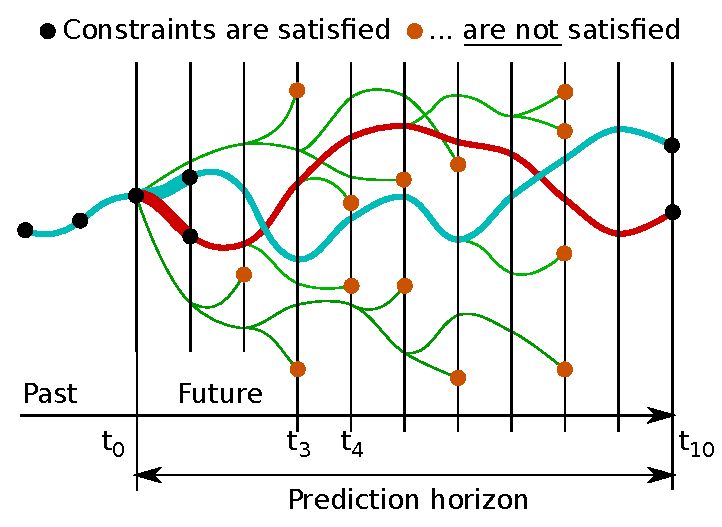
\includegraphics[width=0.7\linewidth]{pics/predictive-horizon.pdf}
  \caption{Predictive horizon based computer simulation}
  \label{fig:hor}
\end{figure}

In order to implement the computer simulation on PCFs representation of RDDESU, data structures for multisets and a default strategy modification are to be designed, and operations within construction of logical inferences are to be implemented.  The latest version of our automatic theorem proving (ATP) software (provers) have RAM (Random Allocated Memory) allocation engines efficiently implementing indexing over the sets of terms. Filter operations for multisets have the similar specifications. Items of the multisets are similar to term and atom in sense of data representation. Special subroutines will be programmed to account specific properties of multisets, their elements and relations, making multiset manipulations memory and time efficient.

The inference engine is to be adjusted with new modifiers and guides to support time and RAM efficient application of operations, filters and constraints as well as representation of grammars over the multisets. The default strategy can be modified with adding each rule (a question) a priority, arranging the rules in an order of application, restricting application of a rule when a pattern is recognized, backtracking the inference in case if criteria have not met within a time interval or a number of the inference rule application, checking constraints to the indexed subsets on the stage of substitution search.


% 7. Component programming (CP) and Python programming language will be the basis of integration of the subsystems. CP allows one to construct reusable pieces of software, which can be used independently of the original development and execution context, resulting in the better maintainability of the source code. Each component have strongly defined interface definition, which is does not change within implementation versions. Component naturally used to wrap subsystems, in our case, models of manufacturing processes, automatic theorem prover, computer simulation and result visualization subsystems. The data used to interchange between subsystems are based on a variants of XML, which allows programmer to control structure content, and Semantic WEB graphs, lists of triples <subject, relations, object>, written in the Turtle syntax, and used for representing input model data.

%The Python programming language is exceptionally useful in implementation of model data structure construction and building scientific environments for investigations. The language has a set of instruments to encapsulate low-level languages, like C, as methods of Python classes. Most used of them are Cython and SWIG (www.swig.org). The last one generates Python modules according to an interface definition language that is similar to C/C++. Using such wrappers allows us to encapsulate high performance code in a flexible research software environment.

%8. The algorithms, which will be used, adapted and devised in the project, have natural OR-parallelism (execution branches of a search algorithm are independent each other) in their implementations on MIMD- (Many Instruction Many Data) cluster computing systems, which are characterized with low speed of communication with comarisson to the computations. In our case the main point of parallelism is computer simulation of scenarios of future, for each process core a scenario is assigned, at each step of simulation condition are checked, in the case of new branches of future the resulting scenarios are executed on the same core or CPU. If there are unbalanced load on cores the balance is periodically reconstructed by moving a tree of scenarios to less load nodes.

%In the same time, for each scenario executed on a CPU a priority could be assigned in the image and likeness of A* algorithm or AND-OR-trees, resulting in the more perspective scenarios calculating early. The priority is calculated by special trajectory evaluation routines. For example, a depth-first heuristic could set better priority for the scenarios, which the greatest time moment are nearer to the horizon constraint. From other hand side, we can account the amount of the additional resources spent to neutralize uncertainty events and prefer that spending less resources. With these priorities we will speed up the time of execution.

% Results
% 2021. New programmatic engines (data structures, inference engines, indexing etc.) for manipulating multisets with automatic theorem proving; techniques and transformation software for representation of RDDESU with SysML diagrams; methods of representation of manufacturing processes as RDDESU; computer supervisor control synthesis software for RDDESU with external uncertainties.
% 2022 Improvement of computer software with control extended to internal events and computer simulation; technique of control synthesis on the base of computer simulation with constraints; publishing results of performance comparison and test results on real problems; adaptation of the technique to the real-world manufacturing control.
% 2023 High-performance variant of the computer simulation software, which includes 1. Cluster node manager distributing subtasks according to heuristic assessment of prospects per scenario. 2. Comparison with the previous uniprocess version. 3. Techniques of assessment of the reserved resources according to the synthesized control. 4. Testing results of the synthesized control on real-world manufacturing processes.

%Ожидаемые результаты научного исследования и их научная и прикладная значимость / Expected results of the research and their theoretical and applied value


% Имеющийся у международного научного коллектива научный задел по проекту, наличие опыта совместной реализации проектов (указываются полученные ранее результаты, разработанные программы и методы)/ The progress of the research, which already exists of the international collective (Notifying early results, developed programs and methods)


% Matrosov Institute for System Dynamics and Control Theory, Siberian Branch or Russian Academy of Sciences (ISDCT SB RAS) have been organized as an institution primary dealing with differential equations, control theory (CT), artificial intelligence (AI). Since the establishment a number of schools were organized. At present the following directions, related to the topic of the research are being developed.

% 7. ISDCT SB RAS team has great deal of experience in constructing complex programming systems by combining various software components and modules. For example, a decision support systems (DSS) has been constructed for forest resources rational consumption DSS was implemented. The decisions are the set of three scenarios of a forest harvesting control, fire prevention, finances spent to insect control, etc. corresponding a set of qualitative and quantitative constraints. The scenarios were calculated with model of the forest dynamics. The model is constructed by a Prolog inference machine with respect to the information describing the forest resources condition. Another example of DSS is system for generation of routine maintenance of petroleum equipment on the base of its structure analysis and modeling of kinetics and dynamics of material destruction.

% For knowledge bases development support by a domain specialist, a visual domain definition software has been developed. The software realizes whole set of models of Model-Driven Architecture in the design process: from Computationally-Independed model of a domain of a technical system to the CLIPS and OWL2 sources of the knowledge base generation.

%8. Since 2003 cluster computing is one of the primary research direction in ISDCT SB RAS. The following directions are developed: intelligent cluster administration, improving cluster utilization, devising new tools for automation of parallel versions of computer software construction, namely ORLANDO tools [8]. ORLANDO tools allows programmer to represent a set of  dependable modules as a network, describe additional constraints, and then construct an execution plan and schedule on a cluster, which features are also described. The instrumental tools are used by users to intensify their software development.

\section{Future Work}
\label{sec:disc}

Expected results and their practical values are expected to be as follows:
\begin{enumerate}
\item A technique for representation of various aspects of RDDESU as a complex of models will be developed, data structures for representation of the complex will be proposed.
\item For a visual representation of the aspects, a corresponding standard visual representation (\emph{e.g.} within UML, SysML, CMMN notations) and its editing software will be adopted, and a usage technique will be proposed.
\item A software for a) transformation of the visual models to the internal representation will be realized as structured logical objects, encapsulating transformational knowledge and algorithms; b) methods of building supervisors for the DES will be developed based on the use of means of automatic proving theorems in PCF-calculus (calculus of positively-constructed formulas).
\item The authors’ technique of constructive inferences constructions on the base of PCFs will be improved to support multisets and operations over them as first class objects, being subject of the inference, as well as new modifications of the default strategy of the inference search will be obtained, making the inference be more productive; a parallel versions of new strategy will be devised for cluster computing systems.
\item Methods, developed in the project will be organized as a modular software for carrying on scientific research (scenario generation, computer simulation and criteria assessment) in the field of RDDESU, intelligent user interfaces for process control will be devised, as well as various means of the result representations.
\item For application aspect of the research, techniques of the near-to-real manufacturing process formulation as complex of visual models will be developed, examples of the formulation will be presented and their control synthesized.
\item An extensive testing of the synthesized control on testing and near-to-real examples will be carried out to assess the performance and other characteristics with the competing approaches.
\end{enumerate}

In parallel, the following investigations will be carried on in LNHU. The work is related to the adaptation the RDDESU approach to the real-world classes of manufacturing process.
\begin{enumerate}

\item Research of resource-driven multi-objective optimization method based on the resource-driven game model, a new efficient method for obtaining the optimal set point (the optimal solution) and the coordinating multi-objective strategy will be developed. %Thanks to usage of the resource-driven based optimization, the new strategy should overcome the constraints among the multiple objectives of the existing strategy to improve the efficiency of searching optimal set point.
\item Research of distributed predictive control for RDDESU with regards of industrial scale and complexity.
%For the discrete-event systems with uncertainties of the resource volume and the requirements, the resource-driven game model is regarded as the predictive model and the distributed predictive control method will be proposed based on this model. The control performance of the system is analyzed.
\item The establishment of visualization model of typical industrial process of ethylene and polypropylene production.
%The characteristics, process flow and unit parameters of typical ethylene and polypropylene production processes will be analyzed on the base of the proposed approach. The models of resource-driven discrete-event system are used to establish the visualization model (notation) of ethylene and polypropylene production processes for the developed software environment.
\item Application of the proposed control algorithm of RDDESU to typical petrochemical processes accounting the uncertainties.
%The uncertainties on resource allocation and the demands of ethylene and polypropylene production processes are analyzed. The distributed predictive control method of resource-driven discrete-event system will be applied to the actual ethylene and polypropylene production process. The application of the synthesized control strategy will guarantee the values of the output coefficients of ethylene and polypropylene to be within prescribed intervals when functioning under the impact of the uncertainties. The comparison of the control effect between distributed predictive control algorithm and the conventional control algorithm will be carried on, the results will be visualized.
\end{enumerate}

The expected results will discover new opportunities for rising level of commodities batch manufacturing control, as well as service. The project expands the theoretical knowledge in DES, GT, ATP, constraint programming, which are the fields of artificial intelligence, as well as manufacturing modeling. The produced software could be used to construct CAE/CAM (Computer-aided engineering/Computer-aided manufacturing) systems for concrete enterprises.

\section{Conclusion}
\label{sec:conc}

The problem of construction of an automated research software for investigating properties and control synthesis for a complex large-scale industrial dynamical system is considered in the paper.  The control must hold the system within prescribed set of constraints describing admissible states, while the system is affected by uncertainties of various kind.  A system model general design is proposed, where the uncertainties are divided onto external, caused by competitors and counterparties, and internal occurring at place being result of utility shortage, equipment failure, staff absence.  The theories of Discrete-event systems and Resource-based games are used in the representation of the industrial system batch manufacturing processes, which are a general case.

The following results are to be obtained: 1) a resource-driven game based model of a manufacturing process accounting competitive environment of an enterprise will be developed, 2) techniques of control synthesizing minimizing deviations of the process execution due to perturbation, 3) new strategies of inference search for positively constructed formulae, 4) new formalized knowledge for model conversion and interpretation represented as objects, 5) computer simulation and visualization system implementing the above mentioned methods and techniques. The scientific novelty is justified the usage of data close to real, application of the transformational technologies in software that allow one to deal with more complex models and account more data. The theoretical results could be used to construct decision support systems for engineering manufacturing processes, assessment of the robustness of the synthesized control.

The collective has a certain foundation on the control synthesis, modeling and optimization of production scheduling and planning, description and management method for uncertainties occurring in industrial process. For a concrete manufacturing process, techniques for formulation of the production scheduling model and dealing with the internal uncertain factors of manufacturing process based on the chance constraint programming and fuzzy theory \cite{b6} have been developed. For the typical concrete manufacturing process with multivariate, strong coupling, large time delay and multi-time scale, a set of systematic and practical optimization and control schemes are proposed by the two-layer way, in which the upper layer adopts the set-point optimization method with the slow sampling time and the down layer adopts the distributed predictive control with the fast sampling time. In view of this, some factors such as the change of the raw material, the lifetime drop of the total load, external environment and the associated coupling among the sub-systems that influence the control quality of the system in industrial control can be overcomed, the control performance can be improved, the product quality and economic benefit can be increased.

The enrichment of the two-level standardized model of manufacturing process with resource-driven representation and parts simulating internal disturbances will add a third level of execution dynamics under a control.  The manufacturing process naturally is being under impact of various uncertainties (perturbations) such as delay of resource supply, the equipment breakdown, temporal lack of labor, sudden production need, requiring equipment occupation on the urgent tasks. These uncertainties are modeled either ``in overage'', \emph{e.g.}, as probability to finish production on time, or an average resource loss (see section \ref{sec:rel-works}).  We suggest rectify these approaches with synthesis (on the third level) of an optimal control supervisor automata preventing some events to happen, or as a result of computer simulation in discrete time. The control is synthesized as a sequence of actions of a trajectory holding imposed constraints in virtual timescale during a significant time period.

\section*{Acknowlegements}
\label{sec:ack}

The research is being supported by Russian science foundation, grant No. 21-41-00022.

\begin{thebibliography}{999}
    % \makeatletter
    % \def\@biblabel#1{[#1]}
    % \makeatother

    \bibitem{rbg} I.~Sheremet. ``Resource-based games,'' CEUR-WS proceedings, Vol.~2638, Proceedings of the 2nd International Workshop on Information, Computation, and Control Systems for Distributed Environments, Irkutsk, Russia, July~6-7, 2020, pp.~234-251.
    \bibitem{andres} A.~A.~Osorio-Londoño, J.~C.~Naranjo-Valencia, G.~Calderón-Hernández, ``Training and its influence on competitive strategy implementation,'' Human Resource Development Quarterly, 31, 2, 2019, p~149-172. \doi{10.1002/hrdq.21381}
    \bibitem{ahmed}M.~U.Ahmed, M.~M.~Kristal, M.~Pagell, T.~F.~Gattiker. ``Building high performance supply-chain relationships for dynamic environments'', Business Process Management Journal, Vol.~26, No.~1, 2019. p.~80-101. \doi{10.1108/BPMJ-05-2018-0139}
    \bibitem{gomes}  D.~A.~Gomes, J.~Saúde, ``Mean Field Games Models—A Brief Survey,'' Dyn. Games Appl. 4, 2014, p.~110–154. \doi{10.1007/s13235-013-0099-2}
    \bibitem{dux} X.~Du, Y.~Xi, S.~Li. ``Distributed Model Predictive Control for Large-scale Systems,'' American Control Conference, 2001, Proceedings of the 2001, IEEE, 2001, 4, p.~3142-3143.
    \bibitem{lis} S.~Li, Y.~Zhang, Q.~Zhu. ``Nash-optimization Enhanced Distributed Model Predictive Control Applied to the Shell Benchmark Problem,'' Information Sciences, 2005, 170(2), p.~329-349.
    \bibitem{liuy} Y.~Liu, X.~Luo, F.~Xu. ``Global Coordination and Stability Analysis for Distributed Model Predictive Control System.'' Journal of Chemical Industry, 2013, 64(4), p.~1318-1331.
    \bibitem{venkat} A.~N.~Venkat, J.~B.~Rawlings, S.~J.~Wright. ``Stability and Optimality of Distributed Model Predictive Control,'' In: Proceedings of the 44th IEEE Conference on Decision and Control, and the European Control Conference. Seville, Spain: IEEE, 2005, p.~6680-6685.
    \bibitem{asadi} E.~Asadi, A.~Richards. ``Scalable Distributed Model Predictive Control for Constrained Systems,'' Automatica, 2018, 93, p.~407-414.
    \bibitem{zouyy} Y.~Y.~Zou, X.~Su, S.~Y.~Li, Y.~G.~Niu, et al. ``Event-triggered Distributed Predictive Control for Asynchronous Coordination of Multi-agent Systems,'' Automatica, 2019, 99, p.~92-98.
    \bibitem{lijn} J.~N.~Li, J.~L.~Ding, T.~Y.~Chai, C.~Li, L.~L.~Frank. ``Nonzero-sum Game Reinforcement Learning for Performance Optimization in Large-scale Industrial Processes,'' IEEE Transactions on Cybernetics, 2019, Early Access Article.
    \bibitem{lidewei} L.~Dewei, X.~Yugeng, Zh.~Pengyuan. ``Constrained Robust Feedback Model Predictive Control for Uncertain Systems With Polytopic Description,'' International Journal of Control, 2009, 82(7), p.~1267-1274.
    \bibitem{b6} Y.~Wang, X.~Jin, L.~Xie, Y.Zhang, S.~Lu. ``Uncertain Production Scheduling Based on Fuzzy Theory Considering Utility and Production Rate,'' Information 2017, 8, 158.
    \bibitem{b1} A.~Feoktistov, R.~Kostromin, I.~Sidorov, S.~Gorsky, G.~Oparin. ``Multi-agent Algorithm for Re-allocating Grid-resources and Improving Fault-tolerance of Problem-solving Processes'', Procedia Computer Science, Vol.~150, 2019, pp.~171-178. \doi{10.1016/j.procs.2019.02.034}
    \bibitem{b3} E.~Cherkashin, A.~Shigarov, V.~Paramonov. ``Representation of MDA Transformation with Logical Objects,'' 2019 International Multi-Conference on Engineering, Computer and Information Sciences (SIBIRCON), Novosibirsk, Russia, 2019, p.~0913-0918. \doi{10.1109/SIBIRCON48586.2019.8958008}
    \bibitem{b2} E.~Cherkashin, I.~Terehin, V.~Paramonov, V.~Tertychniy, ``New transformation approach for Model Driven Architecture,'' Proceedings of the 35th International Convention MIPRO, Opatija, 2012, p.~1082-1087.
    \bibitem{tsyoo} T.-S.~Yoo, S.~Lafortune. ``A General Architecture for Decentralized Supervisory Control of Discrete-Event Systems,'' Discrete Event Dynamic Systems. 2002. Vol.~12, Iss.~3. p.~335-377. \doi{10.1023/A:1015625600613}
    \bibitem{supdes} A.~Davydov, A.~Larionov, N.~Nagul. ``Logic Inference Based Construction of a Supervisor for a Discrete Event System,'' CEUR-WS proceedings, Vol. 2638, Proceedings of the 2nd International Workshop on Information, Computation, and Control Systems for Distributed Environments, Irkutsk, Russia, July~6-7, 2020,  p.~53-67.
    \bibitem{langdes} A.~Davydov, A.~Larionov, N.~Nagul. ``The Construction of Controllable Sublanguage of Specification for DES via PCFs Based Inference,'' CEUR-WS proceedings, Vol.~2638, Proceedings of the 2nd International Workshop on Information, Computation, and Control Systems for Distributed Environments, Irkutsk, Russia, July~6-7, 2020, p.~68-78.
    \bibitem{b4} I.~Bychkov, A.~Davydov, M.~Kenzin, N.~Maksimkin, N.~Nagul and S.~Ul’yanov, ``Hierarchical Control System Design Problems for Multiple Autonomous Underwater Vehicles,'' 2019 International Siberian Conference on Control and Communications (SIBCON), Tomsk, Russia, 2019, p.~1-6, \doi{10.1109/SIBCON.2019.8729592}
    \bibitem{b5} A.~Davydov, A.~Larionov, N.~Nagul, ``PCF-based Formalization of the Parallel Composition of Automata,'' Proceedings of the 1st International Workshop on Information, Computation, and Control Systems for Distributed Environments, ICCS-DE 2019, Irkutsk, Russia, July 8-9, 2019. CEUR Workshop Proceedings. p.~29-41.
    \bibitem{b7} E.~Cherkashin, S.~Badmatsyrenova, A.~Popova, I.~Vladimirov. ``An Optimal Control Module of Sustainable Natural Resources Consumption Control Synthesis for Decision Support Systems,'' Proc. of 37th International Convention on Information and Communication Technology, Electronics and Microelectronics, MIPRO 2014 - Proceedings, 2014, p.~1100-1105.
%    \bibitem{b8} Feoktistov A., Gorsky S., Sidorov I., Bychkov I., Tchernykh A., Edelev A. (2020) Collaborative Development and Use of Scientific Applications in Orlando Tools: Integration, Delivery, and Deployment. In: Crespo-Mariño J., Meneses-Rojas E. (eds) High Performance Computing. CARLA 2019. Communications in Computer and Information Science, vol 1087. Springer, Cham

\end{thebibliography}

\end{document}
%%% Local Variables:
%%% mode: latex
%%% TeX-master: t
%%% End:

-------------------
Reviewer #1 Comments

Well structured and written manuscript on interesting and contemporary topic. The following corrections are required:

*1. Language improvement. The paper needs language improvement, which includes correcting mistakes regarding use of tenses, articles and sentences' construction. Careful reading of the whole manuscript is advised.

*2. According to conference template, there is no need to include index terms after abstract.

*3. References should be carefully read and typos should be corrected (e.g. names in reference no. 2).


--------------------
Reviewer #2 Comments

This paper has an interesting, broad and applicable target, which leads to many possibilities to develop solutions in related scientific and professional projects. It provides a valuable insight in the problem of uncertainty within large-scale systems which are resource and event-driven, with the detailed review of literature related to the problem, existing solutions and scientific contributions in the field.

Authors should make some minor changes in paper:

*1. Paper title should be written with Title Case.

*2.    Section III (currently entitled “Technology supporting research) should have a different title. Current title of the section is confusing. Since the content of the section is related to the proposed approach, it is suggested that title would be: The Proposed Approach.

*3. Authors should be very careful with abbreviations. First occurrence of each abbreviation should be accompanied with the complete word phrase. Mostly, authors were accurate, but sometimes there is some abbreviation unexplained, such as ISDCT SB RAS.

*4. Authors should avoid personal-related words, such as “The colleagues will perform…”, or “Chinese colleagues already have”… It is better to make impersonal form of sentences, such as “It is planned to be performed…”.

*5. Each section should be numbered with Roman numbers, except references. Currently, the Conclusion section does not have the numbering.

*6. Section IV is related to the planned future work, but it is not a discussion of obtained results. Therefore, the section title should be adjusted to the content. It is proposed to have the title “Future Work”.

Non-mandatory suggestions for improvements:

It would be beneficial to have some diagrams (visualizing the components of the planned system to be developed). This way, the paper would be more readable and understandable.
